\documentclass[a4paper,handout]{beamer}

\usepackage{amssymb}
\usepackage{latexsym,amssymb,amsmath,amsbsy,amsopn,amstext,color,multicol}
\usepackage{upgreek}
\usepackage{graphicx,wrapfig,fancybox,watermark,picins}
\usepackage{pgf,pgfarrows,pgfnodes,pgfautomata,pgfheaps,pgfshade}
\usepackage{graphics}
\usepackage{movie15}
\usepackage{hyperref}
\usepackage{bibentry, natbib}

\usefonttheme[professionalfonts]{serif}


\usepackage[red,numbers,minimal]{beamerthemeHongKong}

\hypersetup{pdfpagemode=FullScreen}

\begin{document}

% reference style
\bibliographystyle{ieeetr} 
%reference lib
\nobibliography{refs}

\title[Tutorial 8]{Tutorial 8 the Mid-term Test}
\author[COMP210]{Qu Xiaofeng, Teaching Asistant}
\institute{COMP210\\Discrete Structure}
\date{\today}
\frame{\titlepage}


\section*{Table of Contents}
\frame {
\frametitle{\secname}
\tableofcontents
}

\section{Problems}

\subsection{Problem 1 (10pt)}
\begin{frame}[t]
  \frametitle{\subsecname}
\textit{A TVB television poll of 151 people found that 68 watched ``Lives of Omission'', 61 watched ``Men with no shadows''; 52 watched ``Be home for dinner''; 16 watched both ``Lives of Omission'' and ``Men with no shadows''; 25 watched both ``Men with no shadows'' and ``Be home for dinner''; 19 watched both ``Lives of Omission'' and ``Be home for dinner''; and 26 watched none of these shows. How many persons watched all three shows? Justify your answer.}
\begin{align*}
A 	&=\{people\ who\ watched\ ``Lives\ of\ Omission''\} &= 68\\
B 	&=\{people\ who\ watched\ ``Men\ with\ no\ shadows''\} &= 61\\
C 	&=\{people\ who\ watched\ ``Be\ home\ for\ dinner''\} &= 52\\
\end{align*}
\end{frame}

\begin{frame}[t]
  \frametitle{\subsecname\ cont.}
\begin{align*}
A \cap B = 16\ \ \ \ \ \ \ \ B \cap C = 25\ \ \ \ \ \ \ \ A \cap C = 19\\
\overline{A \cup B \cup C} = 26\ \ \ \ \ \ A \cup B \cup C = 151 - 26 =125
\end{align*}
\begin{align*}
To\ find\\&
 &A\cap B \cap C &=(A\cup B\cup C) +(A\cap B) +(B\cap C) +(A\cap C)\\
 	& & &\ \ \ -A -B -C\\
	& & &=125 +16 +25 +19 -68 -61 -52 =4
\end{align*}
\hfill $\blacksquare$
\end{frame}

\subsection{Problem 2 (20pt)}
\begin{frame}[t]
  \frametitle{\subsecname}
  \textit{True or False:}
  \begin{itemize}
  \item Let A = \{1, 3, 5\}, B = \{3, 4\}, A-B=\{5\}
  	 \hfill \alert{False} \\
  \item If $ p\rightarrow q $, then $ \neg (p\wedge \neg q) $
  	 \hfill \alert{True} 
  \item $\exists x$, s.t., $x^2+x+1<0$
  	 \hfill \alert{False} 
  \item Assume the musical will be scheduled if and only if both Jay and Marry show up on time. Since Jay is not here, the musical will be canceled.
  	 \hfill \alert{True} 
  \item Let the domain and co\textendash domain be real numbers. Then, f(x)=3x is bijective.
  	 \hfill \alert{True}
  \end{itemize}
\end{frame}

\begin{frame}[t]
  \frametitle{\subsecname\ cont.}
  \textit{True or False:}
  \begin{itemize}
  \item If f(x) is onto, its inverse function exists
  	 \hfill \alert{False} 
  \item Relation \{(1,2), (2,1)\} is reflexive.
  	 \hfill \alert{False} 
  \item If $\lfloor x\rfloor=\lceil x \rceil$, then x is an integer number
  	 \hfill \alert{True} 
  \item $\forall y \in Z^+$, x mod y is non-negative
  	 \hfill \alert{True} 
  \item A relation can be both anti-symmetric and symmetric.\\
  	 \hfill \alert{True}
  \end{itemize}
  \hfill $\blacksquare$
\end{frame}

\subsection{Problem 3 (30pt)}
\begin{frame}[t]
  \frametitle{\subsecname}
  \textit{Prove or disapprove the following statements:\\ 
  $\;$ \\
  a. Let $H_k = 1+\frac{1}{2}+\frac{1}{3}+\cdots+\frac{1}{k}$. Then, $\sum^n_{i=1}H_i=(n+1)H_n-n$ for all $n\geq1$.}\\
  $\;$ \\
  
  \alert{True} \hfill prove by induction\\
  $\;$   \\
  
  Base case:\\
  $\sum^1_{i=1}H_i=H_1=1$\ \ \ \ \ \ \ \  $(1+1)\cdot H_1-1=1$\\ $\;$\\ 
  Induction:\\
  For n=k, $\sum^k_{i=1}H_i=(k+1)H_k-k$ is True
\end{frame}

\begin{frame}[t]
  \frametitle{\subsecname\ cont.}
  when\ n=k+1, 
  \begin{align*}
  \sum^{k+1}_{i=1}H_i &= \sum^k_{i=1}H_i + H_{k+1}\\
 			&= (k+1)H_k-k + H_{k+1}\\
 			&= (k+1)(H_{k+1} - \frac{1}{k+1}) - k + H_{k+1}\\
 			&= (k+2)H_{k+1}-(k+1)
  \end{align*}
  \hfill $\blacksquare$
\end{frame}

\begin{frame}[t]
  \frametitle{\subsecname\ cont.}
  \textit{Prove or disapprove the following statements:\\
  $\;$ \\  
  b. $2^n-1$ is prime for all $n\geq1$ }\\
  $\;$ \\    
  \alert{False} \hfill disprove by example\\
  $\;$ \\    
	When n=4,  $2^n-1=16-1=15$ is not a prime number. \\
	\hfill $\blacksquare$
\end{frame}

\begin{frame}[t]
  \frametitle{\subsecname\ cont.}
  \textit{Prove or disapprove the following statements:\\
  $\;$ \\  
  c. There are no positive integer solutions to the equation $x^2-y^2=1$} \\
  $\;$ \\    
  \alert{True} \hfill prove by contradiction\\
  $\;$ \\    
If there exist positive integer x, y, then x+y, x-y are both integers.\\ 
$\Rightarrow$
\begin{columns}
\column{0.5\textwidth}
\[
\begin{cases}x+y=1\\x-y=1
\end{cases}
\]
\column{0.5\textwidth}
\[
\begin{cases}x+y=-1\\x-y=-1
\end{cases}
\]
\end{columns}
\end{frame}

\begin{frame}[t]
  \frametitle{\subsecname\ cont.}
\begin{columns}
\column{0.5\textwidth}
\[
\begin{cases}x+y=1\\x-y=1
\end{cases}
\]
\column{0.5\textwidth}
\[
\begin{cases}x+y=-1\\x-y=-1
\end{cases}
\]
\end{columns}

\begin{columns}
\column{0.5\textwidth}
\centering
$\Downarrow$
\[
\begin{cases}x=1\\y=0
\end{cases}
\]
\column{0.5\textwidth}
\centering
$\Downarrow$
\[
\begin{cases}x=-1\\y=0
\end{cases}
\]
\end{columns} 
$\;$\\
Contradiction.\\ 
$\Rightarrow$ So the hypothesis is false, the original statement is true.\\
\hfill $\blacksquare$
\end{frame}



\subsection{Problem 4 (30pt)}
\begin{frame}[t]
  \frametitle{\subsecname}
\begin{columns}
\column{0.7\textwidth}
  \textit{Draw the graph of the following relations on \{0, 1, 2, 3, 4\}. Determin if they are reflexive, transitive, symmetric, antisymmetric, partial order?\\
a. xRy if $x+y<4$ }
\begin{align*}
xRy &= \{(x,y)\mid x + y < 4\}\\
  &=\{\{0,0\}, \{0,1\}, \{0,2\}, \{0,3\},\\
  & \{1,0\}, \{1,1\}, \{1,2\}, \{2,0\}, \\
  & \{2,1\}, \{3,0\}\}
\end{align*}
\alert{Symmetric} \\ \hfill $\blacksquare$
\column{50mm}
\begin{figure}
\centering
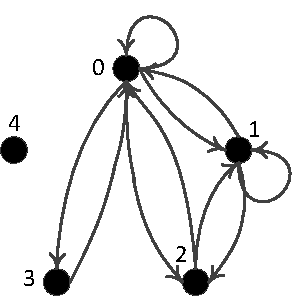
\includegraphics[width=50mm]{im/Tut8p4a}
\end{figure}
\end{columns}
\end{frame}


\begin{frame}[t]
  \frametitle{\subsecname\ cont.}
\begin{columns}
\column{0.7\textwidth}
  \textit{Draw the graph of the following relations on \{0, 1, 2, 3, 4\}. Determin if they are reflexive, transitive, symmetric, antisymmetric, partial order?\\
b. xRy if x is dividable by y }
\begin{align*}
xRy &= \{(x,y)\mid x\equiv 0\ mod(y)\}\\
  &=\{\{0,1\}, \{0,2\}, \{0,3\}, \{0,4\}, \{1,1\},\\ 
  &\{2,2\}, \{3,3\}, \{4,4\}, \{2,1\}, \{3,1\},\\
  &\{4,1\}, \{4,2\}\}
\end{align*}
\alert{Antisymmetric, Transitive} \\ \hfill $\blacksquare$
\column{51mm}
\begin{figure}
\centering
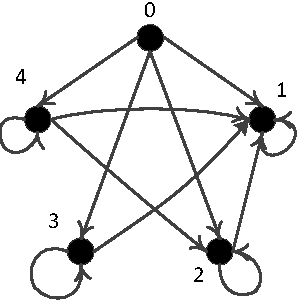
\includegraphics[width=51mm]{im/Tut8p4b}
\end{figure}
\end{columns}
\end{frame}


\begin{frame}[t]
  \frametitle{\subsecname\ cont.}
\begin{columns}
\column{0.6\textwidth}
  \textit{Draw the graphs of the following relations on \{0, 1, 2, 3, 4\}. Determin if they are reflexive, transitive, symmetric, antisymmetric, partial order?\\
c. $\{\{1,1\}, \{2,2\}, \{3,3\}, \{4,4\},$\\
$\{2,3\}, \{3,4\}, \{4,2\}\}$} \\$\;$\\
\alert{Antisymmetric}\\ \hfill $\blacksquare$
\column{51mm}
\begin{figure}
\centering
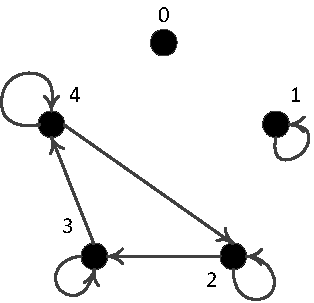
\includegraphics[width=53mm]{im/Tut8p4c}
\end{figure}
\end{columns}
\end{frame}

\subsection{Problem 5 (10pt and 10pt bonus)}
\begin{frame}[t]
  \frametitle{\subsecname}  
  \textit{A plane convex set, subsequently abbreviated to ``convex set'', is a non-empty set X in the plane having the property that if x and y are any two points in X, the straight-line segment from x to y is also in X. The following figures illustrate:}
\begin{columns}
\column{0.5\textwidth}
\begin{figure}
\centering
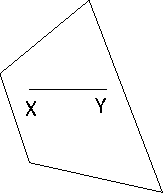
\includegraphics[width=27.5mm]{im/Tut8p5a}
\caption{Convex set}
\end{figure}
\column{0.5\textwidth}
\begin{figure}
\centering
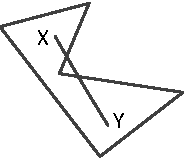
\includegraphics[width=31mm]{im/Tut8p5b}
\caption{Non convex set}
\end{figure}
\end{columns}
\end{frame}

\begin{frame}[t]
  \frametitle{\subsecname\ cont.}  
  \textit{a. Prove that if X and Y are convex sets and $X \cap Y$ is nonempty, then $X \cap Y$ is convex.}\\  $\;$ \\
$ \forall x,y \in X \cap Y$\\ 
Let the point z be on the straight line segment from x to y.\\   $\;$ \\
Since $x,y \in X$, X is convex $\Rightarrow$ $z \in X$ \\  
Since $x,y \in Y$, Y is convex $\Rightarrow$ $z \in Y$ \\   $\;$ \\
$\Rightarrow z \in X \cap Y$ \\ 
\hfill $\blacksquare$
\end{frame}

\begin{frame}[t]
  \frametitle{\subsecname\ cont.}
  \textit{b. Assume the following statement is correct:}\\ 
  \begin{quote} 
  Lemma: Four convex sets are given in the plane. If every three of them have a nonempty intersection, then the intersection of all four sets is also nonempty.
  \end{quote}
  \textit{Prove Helly's theorem: Suppose that $X_1, X_2, \cdots, X_n, n\geq4$ are convex sets, each three of which have a common point. All n sets have a common point.}\\ 
  $\;$\\
\alert{Prove by indcution.}\\ 
$\;$\\
Base step: n=4 true by lemma
\end{frame}

\begin{frame}[t]
  \frametitle{\subsecname\ cont.}
Induction step: true when n=k\\  $\;$\\
now consider n=k+1, for $X_1,X_2,\cdots,X_{k+1}$,\\ 
let $Y_1=X_1\cap X_{k+1},Y_2=X_2\cap X_{k+1},\cdots,Y_k=X_k\cap X_{k+1}$\\
\hfill a total of k sets.\\ 
By (a), all of them are convex. \\ 
consider any 3 sets:\\
$X_i \cap X_{k+1}$, $X_j \cap X_{k+1}$ and $X_l \cap X_{k+1}$ $i, j, l \in \{1,\cdots,k\} $ 
$=X_i \cap X_{j}\cap X_{l}\cap X_{k+1} \neq \phi$ by the base of the induction where we pick four sets $X_i$, $X_{j}$, $X_{l}$, $X_{k+1}$.\\ 
This implies that any three set among $Y_1, Y_2, \cdots, Y_k$ share a common point.\\ 
By induction hypothesis,
$\bigcap_{i=1}^{k+1}X_i=\bigcap_{i=1}^{k}Y_i\neq\phi$ \\
\hfill $\blacksquare$
\end{frame}

\end{document}



